\documentclass{article}
\pdfpagewidth=8.5in
\pdfpageheight=11in

\usepackage{ISRreport}
\usepackage{times}
\usepackage{url}
\usepackage{xcolor}
\usepackage{polski}
\usepackage[polish]{babel}
\usepackage[utf8]{inputenc}
\usepackage[T1]{fontenc}
\usepackage[utf8]{luainputenc}
\usepackage[hidelinks]{hyperref}
\usepackage[utf8]{inputenc}
\usepackage{caption}
\usepackage{indentfirst}
\usepackage{graphicx}
\usepackage{amsmath}
\usepackage{siunitx}
\usepackage{booktabs}
\usepackage{subfig}
\usepackage{pgfplots}
\usepackage{paracol}
\usepackage{gensymb}

\urlstyle{same}
	
\title{Inteligentne Systemy Robotyczne\\ Zadanie sortowania sześcianów}

\author{
Jakub Sikora
\affiliations
numery albumów: 283418 \\
\emails
jakub.sikora2.stud@pw.edu.pl
}

\newcommand{\todo}[1]{\textcolor{red}{\textbf{TO DO:} #1}}

\begin{document}
\maketitle

\section{Opis problemu}
\label{sec:opis-problemu}
\subsection{Treść zadania}
\label{subsec:polecenie}
Należy zaprojektować system sterowania manipulatorem o~sześciu stopniach swobody, wyposażony w~chwytak dwustanowy oraz kamerę RGB-D (Kinect). Na taśmociągu poruszają się różnokolorowe sześciany o~wymiarach 4cm~$\pm$~1cm. Zadaniem robota jest pobieranie żółtych sześcianów poruszających się na czarnym taśmociągu i~układanie ich na palecie o~wymiarach 100cm~x~100cm. Sześciany mają być ustawione na~palecie w~konfiguracji 20x20. 

Szybkość ruchu taśmociągu jest stała i~wynosi $\num{0,1}\frac{m}{s}$ - taśmociąg nie jest sterowany przez projektowany system. Pozycja taśmociągu oraz kamery względem podstawy robota jest znana (określa je projektant systemu). Sześciany spadają pojedynczo na początek taśmociągu co 40~sekund. Ich położenie początkowe i~orientacja są losowe. Szerokość taśmociągu wynosi $\num{0.3}$ m, a~jego długość $\num{1,2}$ m. System rozpoczyna pracę po otrzymaniu komendy \texttt{START}, a~kończy ją gdy paleta się zapełni. Komendy \texttt{START} wydawane są przez zdalnego agenta, którego definiować nie potrzeba. Wymiana palet jest zadaniem innych urządzeń, które nie są pod kontrolą projektowanego systemu.

Stosująć formalizm przedstawiony na wykładzie należy:
\begin{itemize}
    \item określić strukturę systemu w~kategoriach agentów,
    \item dla każdego agenta należy zdefiniować podsystem sterowania, efektory i~receptory wirtualne,
    \item dla tych podsystemów określić:
    \begin{itemize}
        \item automat skończony sterujący ich pracą,
        \item zachowania,
        \item warunki początkowe i~końcowe zachowań,
        \item funkcje przejścia w~postaci matematycznej i~DFD,
        \item zawartość pamięci wewnętrznej oraz buforów wejściowych i~wyjściowych,
        \item krok dyskretyzacji dla każdego podsystemu.
    \end{itemize}
\end{itemize}


\section{Struktura systemu}
\label{sec:struktura}
\subsection{Konfiguracja rzeczywista}
\label{subsec:konfiguracja-urzadzen}

\begin{figure}
    \centering
    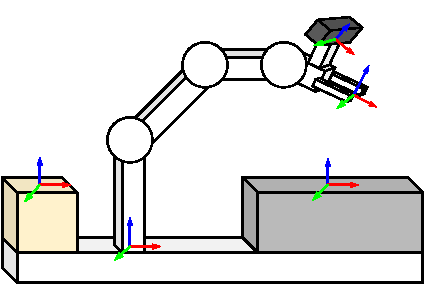
\includegraphics[width=\columnwidth]{figures/ISR-system-overview.pdf}
    \label{fig:srodowisko-robocze}
    \caption{Środowisko robocze projektowanego systemu}
\end{figure}

\subsection{Agentowa struktura systemu}
\label{subsec:agentowa-struktura}

\begin{figure}
    \centering
    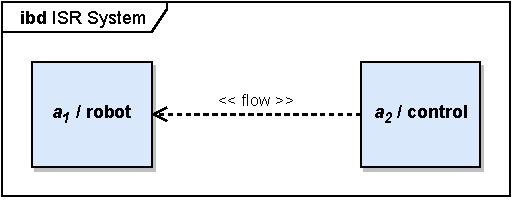
\includegraphics[width=\columnwidth]{figures/ISR-agents.pdf}
    \label{fig:agenty-system}
    \caption{Dekompozycja systemu na agenty}
\end{figure}

\begin{figure}
    \centering
    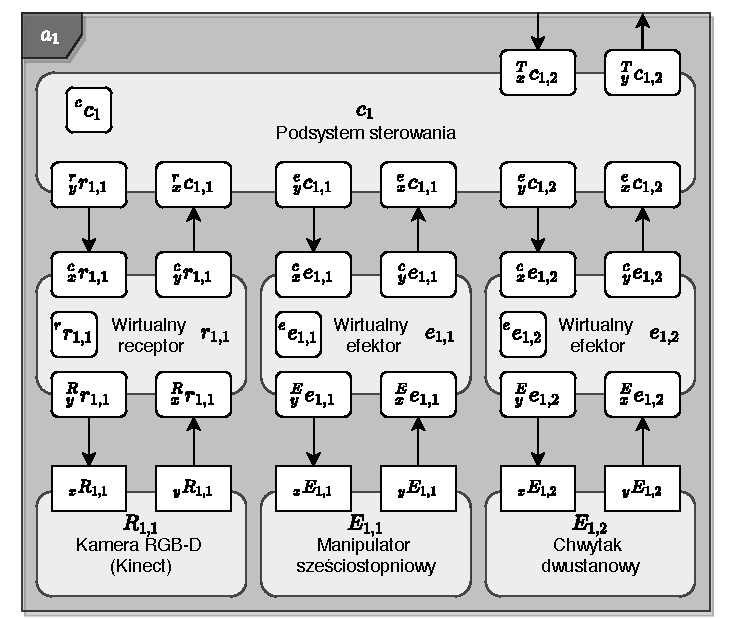
\includegraphics[width=\columnwidth]{figures/ISR-agent-decomposition.pdf}
    \label{fig:dekompozycja-agent-1}
    \caption{Dekompozycja agenta $a_{1}$ na wirtualne i~rzeczywiste receptory i~efektory}
\end{figure}


\bibliographystyle{abbrv}
\bibliography{bibliography}

\end{document}